\section{Introduction}

\def\Z{$\mathbb{Z}$}
\def\R{$\mathbb{R}$}
\newcommand\Wider[2][3em]{%
	\makebox[\linewidth][c]{%
		\begin{minipage}{\dimexpr\textwidth+#1\relax}
			\raggedright#2
		\end{minipage}%
	}%
}
\begin{frame}
	\frametitle{Discrete Time Signal}
	\begin{definition}
		Discrete-time signals are defined only at discrete instants of time. The value (amplitude) can be either continuous or discrete.\\
		$x[k]$ is the value of a signal at the moment $t = kT$
	\end{definition}
	\begin{example}
		\begin{figure}
		\centering
		\includegraphics[width=0.25\linewidth]{Images/Discrete_time_eps_1.eps}
\end{figure}

	\end{example}
\end{frame}
\begin{frame}
	\frametitle{Discrete Time System}
	\begin{block}{Sampling}
		The sampling of a continuous time signal replaces the original continuous signal by a sequence of values at discrete time points.
		\begin{figure}
			\centering
			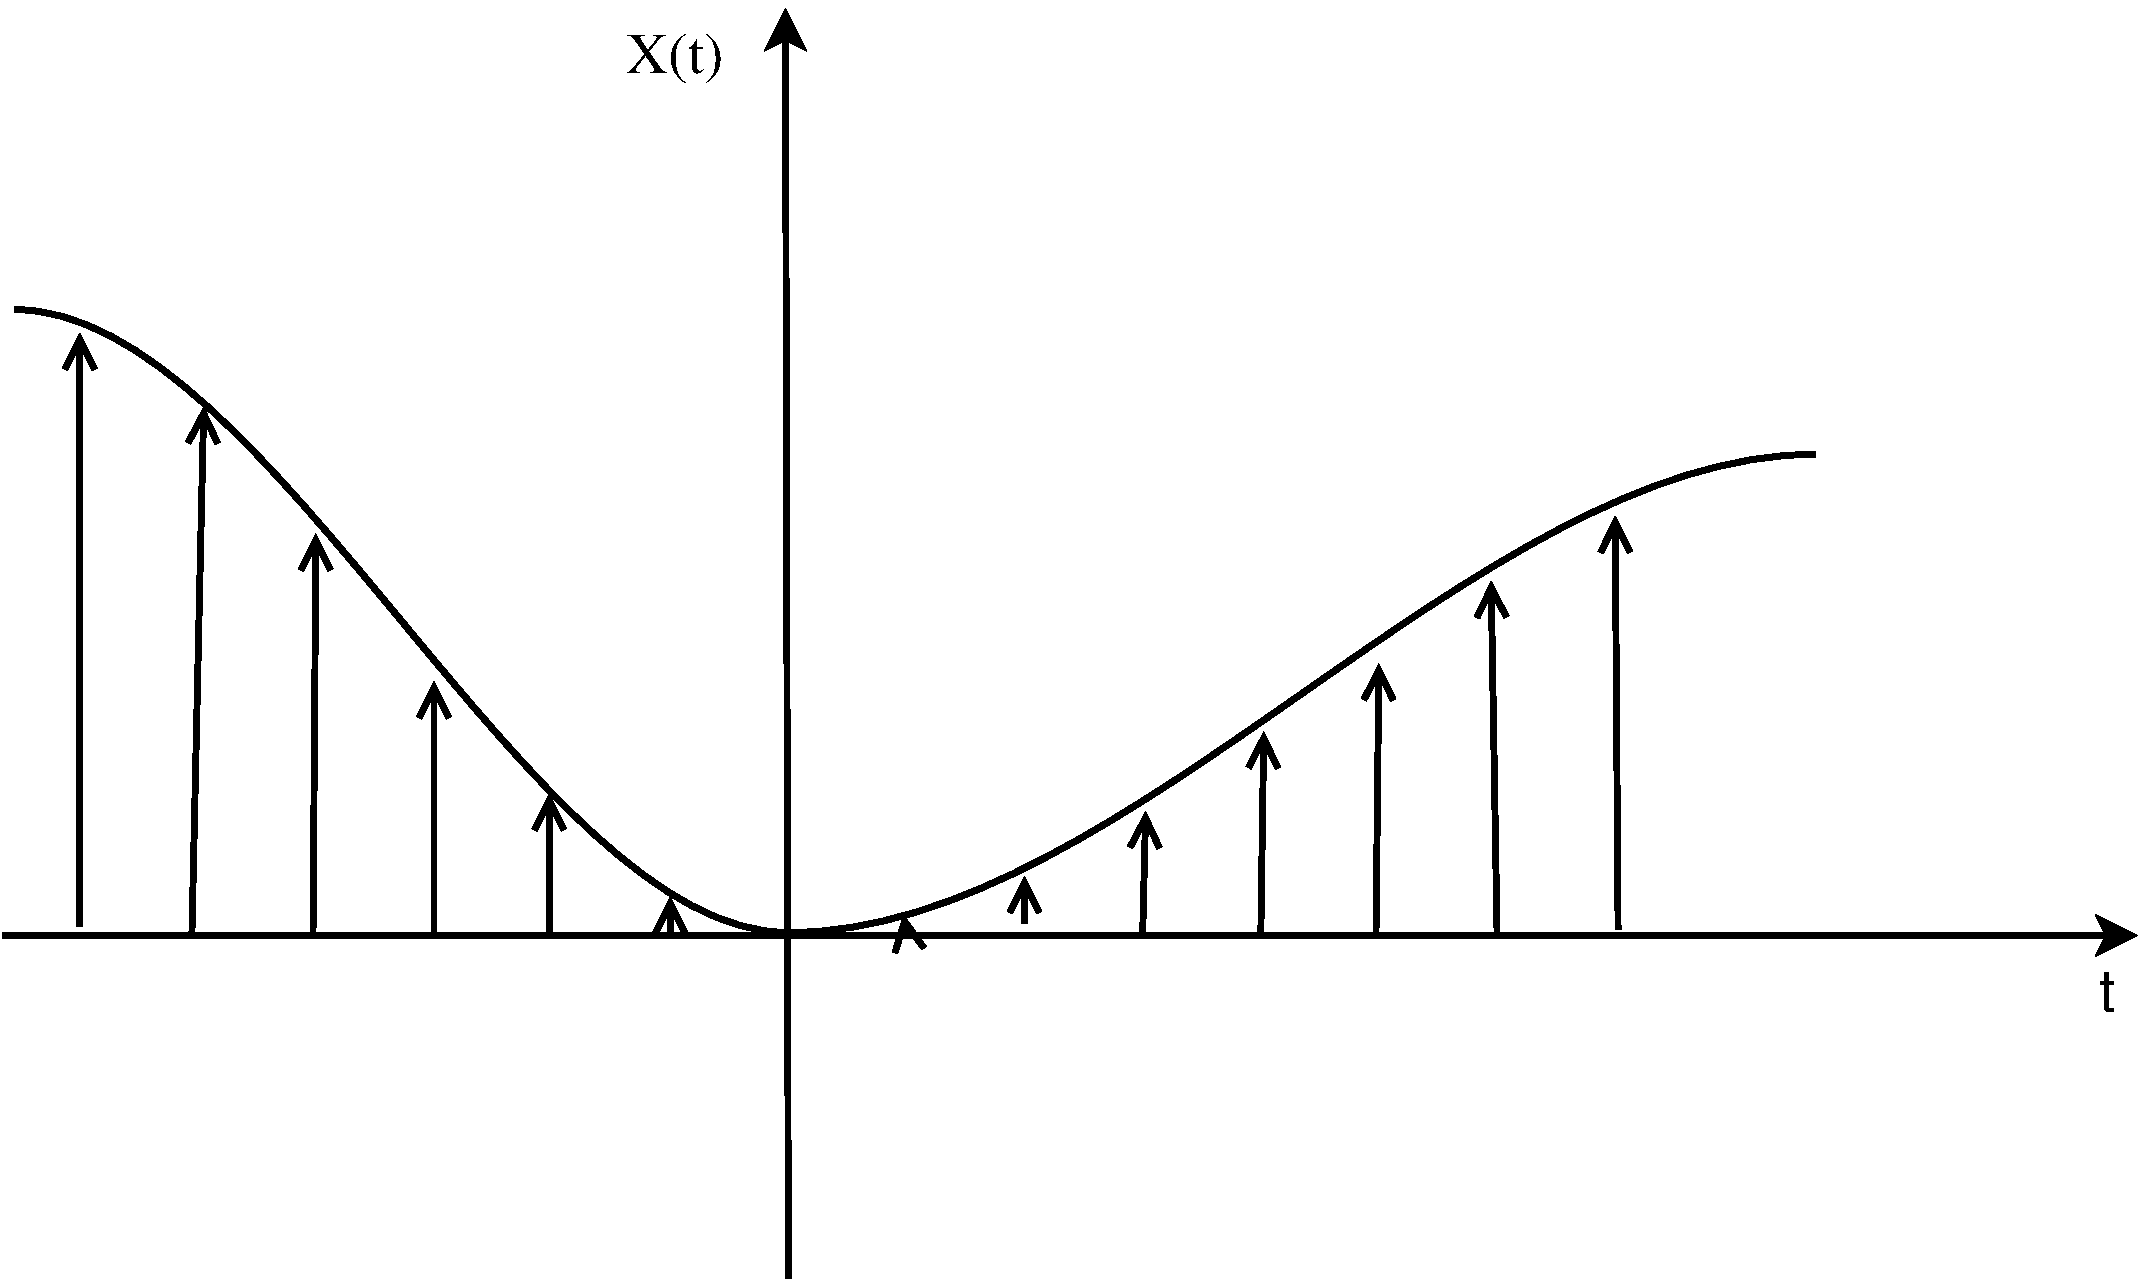
\includegraphics[width=0.5\linewidth]{Images/Discrete_time_eps_4}
		\end{figure}

	\end{block}
\end{frame}
\begin{frame}
	\frametitle{Discrete Time System}
	\begin{definition}
			A linear time-invariant (LTI) discrete time system processes an input vector $u[k]$ to an output vector $y[k]$.\\
	\end{definition}
		\begin{example}
			\begin{figure}
				\centering
				\includegraphics[width=0.7\linewidth]{Images/Discrete_time_eps_2.eps}
			\end{figure}
		\end{example}
\end{frame}
\begin{frame}
	\frametitle{Discrete Time System}
	\begin{block}{How to represent a discrete time system?}
		\begin{itemize}
			\item Block-diagram
			\item State space representation
			\item Difference equation
			\item Impulse response
			\item Transfer function
		\end{itemize}
	\end{block}
	

\end{frame}
\section{Block-diagram}
\begin{frame}
	\frametitle{Block-diagram}
\begin{figure}
\centering
\includegraphics[width=0.7\linewidth]{Images/Discrete_time_eps_3.eps}
\end{figure}


	\vspace{-1.5em}
	\begin{definition}
			A block-diagram is a visual representation of a system. All LTI's (Linear Time Invariant) systems can be constructed using 3 building blocks (memory element, summation element and multiplication element). Note that every memory element corresponds to one state variable.
	\end{definition}
\end{frame}
\begin{frame}
	\frametitle{Building blocks}
	
			\begin{block}{Adder}
			\begin{figure}
				\centering
				\includegraphics[width=0.3\linewidth]{Images/Discrete_time_eps_5.eps}
				
			\end{figure}
%			\include{DT_systems_(11).tex}

			\end{block}
		
		
				\begin{block}{Constant Multiplier}
					\begin{figure}
					\centering
					\includegraphics[width=0.3\linewidth]{Images/Discrete_time_eps_6.eps}
					\end{figure}
				\end{block}
	
			\begin{block}{Delay element}
				\begin{figure}
					\centering
					\includegraphics[width=0.3\linewidth]{Images/Discrete_time_eps_7.eps}
				\end{figure}
			\end{block}
	
\end{frame}
\begin{frame}
	\frametitle{Example: compound interest}
	\begin{itemize}
			\item $ u[k]$:The deposits and withdrawals from the bank account
			\item $ x[k]$:The current balance of the bank account(before deposit and interest)
			\item $ y[k]$: The acquired interest of that year
			\item $ x[k+1]$: The 'next year' balance of the bank account  = current balance + interest + deposits - withdrawals
	\end{itemize}
	 \begin{figure}
			\centering
			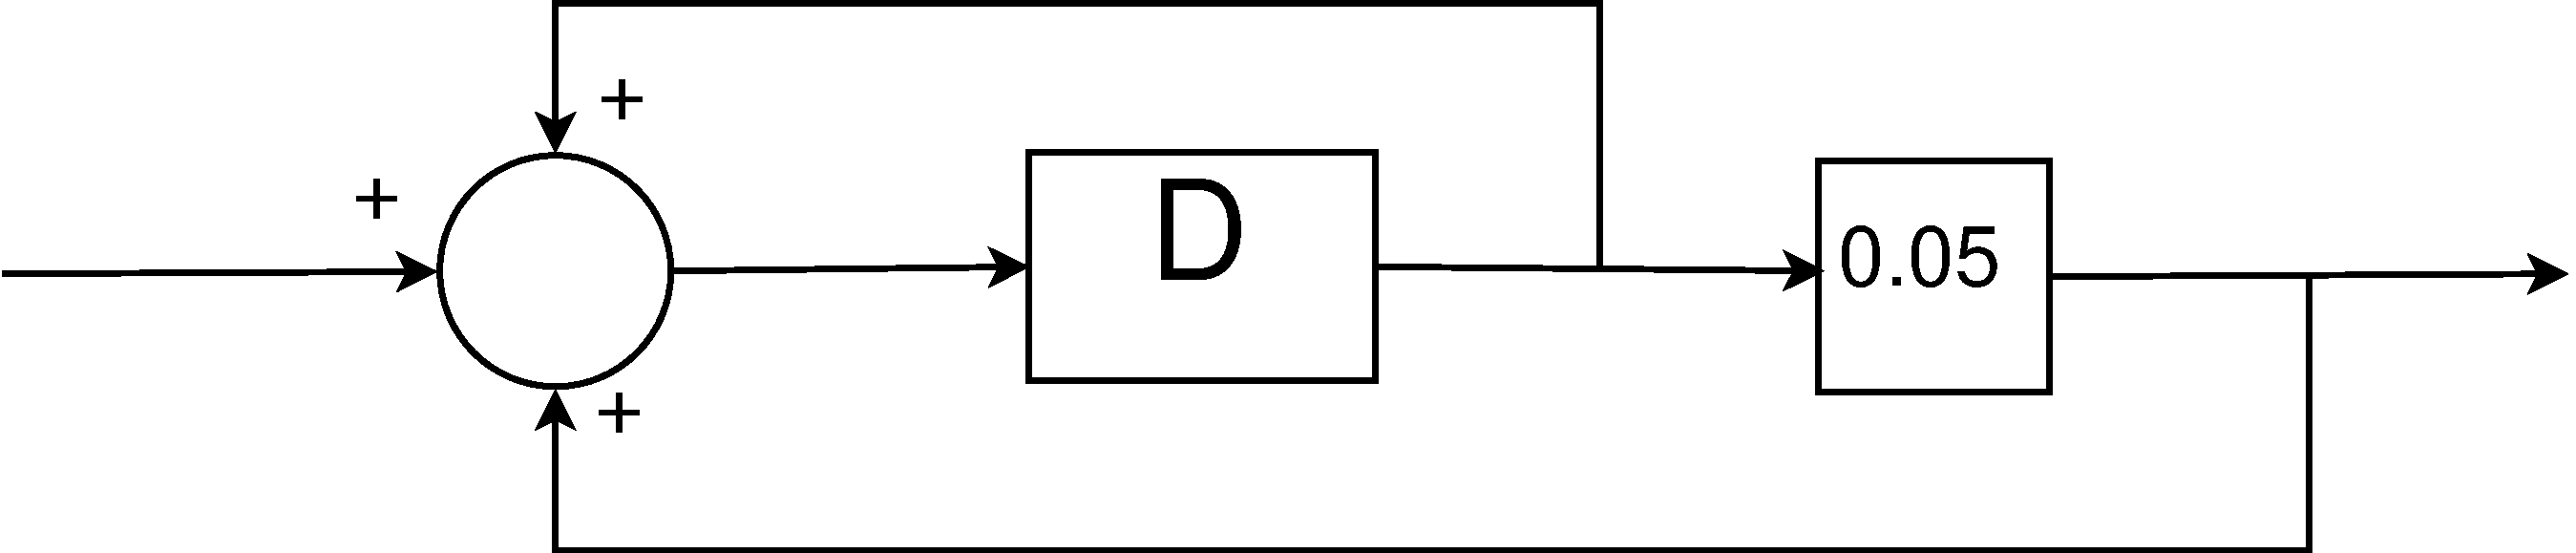
\includegraphics[width=0.7\linewidth]{Images/Discrete_time_eps_14}
		\end{figure}

%	\begin{figure}
%		\centering
%		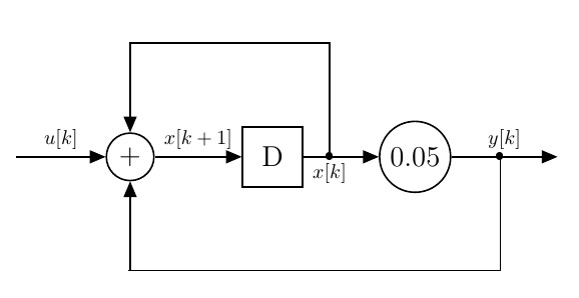
\includegraphics[height=0.4\textheight]{Images/discrete_time_systems_3}
%	\end{figure}
\end{frame}
%\begin{frame}
%	\begin{tabular}{|c|c|c|c|}
%		\hline  $u[k]$& $x[k+1]$  & $x[k]$  & $y[k]$  \\ 
%		\hline  50 & 50 & 0  & 0  \\ 
%		\hline  0 & 52.5  & 50 & 2.5  \\ 
%		\hline  -25 & 30.13 & 52.5 & 2.62  \\ 
%		\hline  0 &  31.63 & 30.13  & 1.51  \\ 
%		\hline  0 & 33.21  & 31.63 & 1.58 \\ 
%		\hline  30 & 64.87 & 33.21  & 1.66 \\ 
%		\hline  0 & 68.12 & 64.87 & 3.24  \\ 
%		\hline  0 & 71.52 & 68.12 & 3.41 \\
%		\hline 
%	\end{tabular}
%	
%
%\end{frame}
\begin{frame}
	\frametitle{Bad block-diagrams}

				\begin{alertblock}{Delay-free loops}
					The issue is that this leads to an implicit connection. 
					$y[k]$ depends on $y[k]$ ,which is not yet known
					You can easily rewrite this in an allowed shape
					$y[k] = u[k]  + 3 y[k] \Longleftrightarrow y[k] = -\frac{1}{2} u[k]$
					\begin{figure}
						\centering
						\includegraphics[height=0.4\textheight]{Images/Discrete_time_eps_10.eps}
					\end{figure}
				\end{alertblock}
\end{frame}
\begin{frame}
	\frametitle{Bad block diagrams}
		\begin{alertblock}{Connecting two outputs without using a sum}
			The issue is that this can lead to inconsistencies.	According to this block diagram the output of the systems S1 and S2 are equal.
			\begin{figure}
				\centering
				\includegraphics[width = 0.5\linewidth]{Images/Discrete_time_eps_15.eps}
			\end{figure}
		\end{alertblock}
\end{frame}
\section{State space representation}
\begin{frame}
	\frametitle{State space representation}
	\begin{definition}
		State space representation of a LTI system:
		\begin{center}
			$x[k+1] = A x[k] + B u[k]$ \\
			$y[k] = C x[k] + D u[k] $ \\
		\end{center}
			State space representation of a LTV system:
			\begin{center}
				$x[k+1] = A[k] x[k] + B[k] u[k]$ \\
				$y[k] = C[k] x[k] + D[k] u[k] $ \\
			\end{center}
%		This state space representation is specific to LTI systems:\\
%		\begin{itemize}
%			\item Linear: it's easy to see these systems are linear
%			\item Time-invariant: the matrices A,B,C,D do not depend on time, if they were time-variant the matrices would be replaced by $A[k], B[k], C[k]$ and $D[k]$.
%		\end{itemize}
	\end{definition}
\end{frame}

\begin{frame}
\frametitle{From block-diagram to state space representation}
\begin{columns}

\begin{column}{0.5\textwidth}
	\begin{block}{Block-diagram}
		\vspace{2.3em}
		\begin{figure}
			\centering
			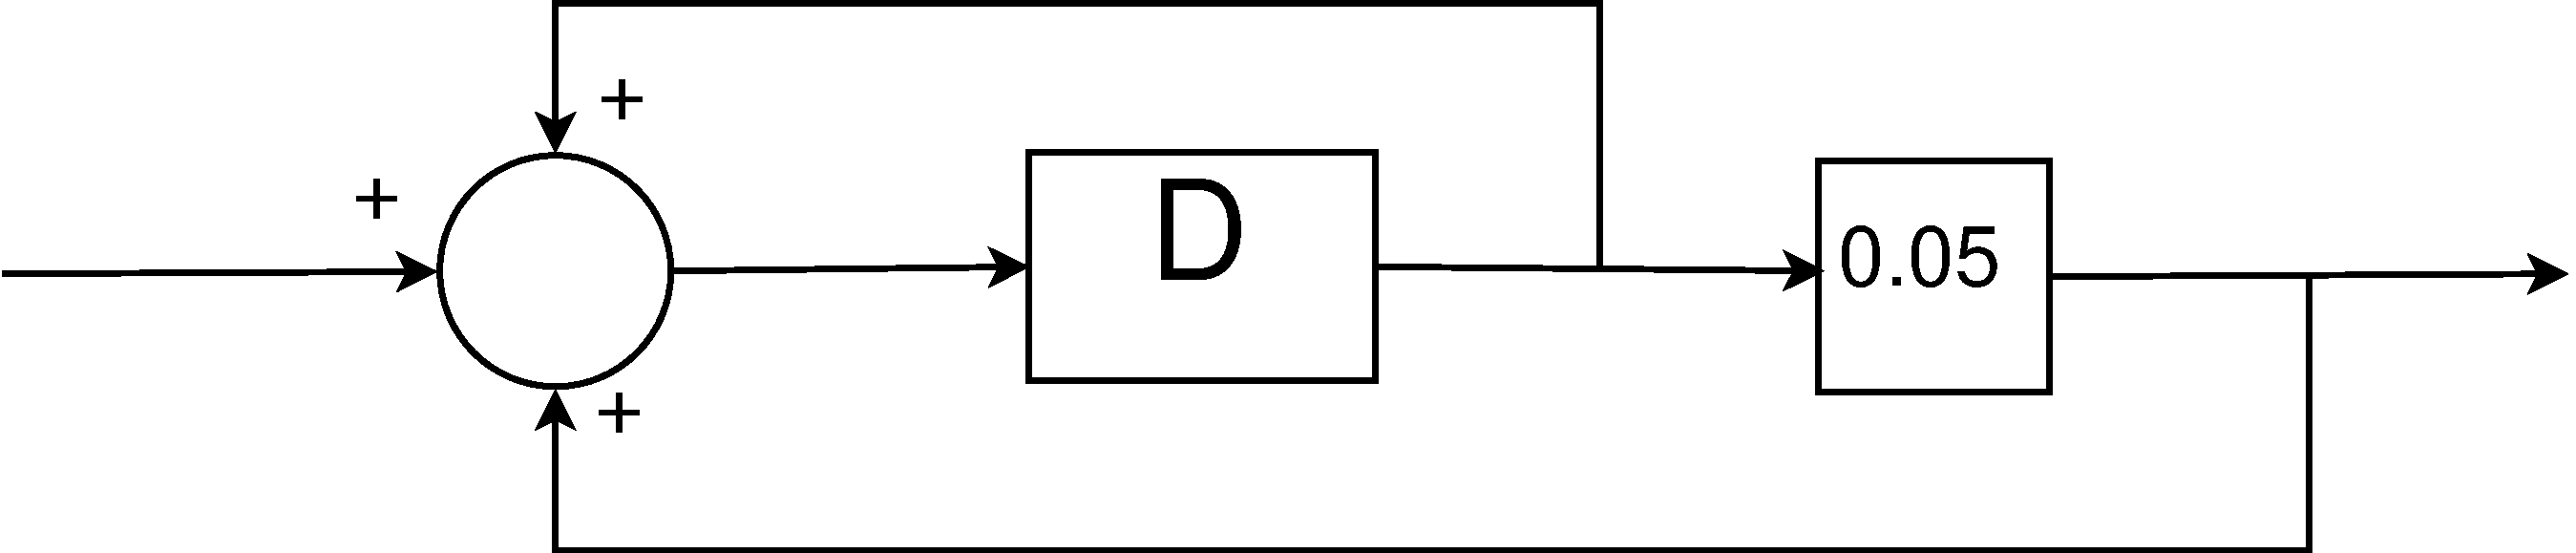
\includegraphics[width=1\linewidth]{Images/Discrete_time_eps_14}
		\end{figure}
		\vspace{2.3em}
	\end{block}
	
\end{column}
\begin{column}{0.5\textwidth}
	\begin{block}{State space representation}
		\begin{enumerate}
			\item Let the output of the memory elements be $x_{i}[k]$. 
			\item So the input of the memory elements are $x_i[k+1]$.
			\item Trace back to retrieve equations for $x_i[k+1] $ and $y_i[k]$.
		\end{enumerate}
		\vspace{-0.5em}
		This results in:
		\vspace{-0.5em}
		\begin{center}
				$x[k+1] = 1.05 x[k] + u[k]$
				$y[k] = 0.05 x[k]$
		\end{center}
	\end{block}
\end{column}
\end{columns}
\end{frame}
\begin{frame}
	\frametitle{From state space representation to block-diagram }
		\begin{example}
				\begin{center}
					$\begin{bmatrix}
						x_1[k+1]\\
						x_2[k+1]\\
						x_3[k+1]
					\end{bmatrix}$
					= 
					$\begin{bmatrix}
						1 & 0 & 0 \\
						0 & 0 & 1 \\
						0 & 3 & 0
					\end{bmatrix}$ 
					$\begin{bmatrix}
						x_1[k+1]\\
						x_2[k+1]\\
						x_3[k+1]
					\end{bmatrix}$
					 +
					$\begin{bmatrix}
					1\\
					0\\
					4\\
					\end{bmatrix}$ $u[k]$\\
					
					$y[k] = 
					\begin{bmatrix}
					5 & 1 & 0
					\end{bmatrix}
					+ 
					\begin{bmatrix}
					1
					\end{bmatrix}
					u[k]$ \\
				\end{center}
		\end{example} 
		
	
\end{frame}
\begin{frame}
	\frametitle{From state space space representation to block-diagram}
	\begin{block}{Step 1}
		First add a delay element for every state $x_i[k]$.
		\begin{figure}
			\centering
			\includegraphics[width=0.35\linewidth]{Images/Discrete_time_eps_11.eps}
		\end{figure}
	\end{block}
\end{frame}
\begin{frame}
	\frametitle{From state space space representation to block-diagram}
	\begin{block}{Step 2}
		Determine the input for every state $x[k+1]$ from the matrices A and B, as a combination of the states $x_i[k]$ and inputs $u[k]$.
		\begin{figure}
			\centering
			\includegraphics[width=0.5\linewidth]{Images/Discrete_time_eps_12.eps}
		\end{figure}
	\end{block}
\end{frame}
\begin{frame}
	\frametitle{From state space space representation to block-diagram}
	\begin{block}{Step 3}
		Determine the outputs y[k] in the same way with the matrices C and D.
			\begin{figure}
				\centering
				\includegraphics[width=0.7\linewidth]{Images/Discrete_time_eps_13.eps}
			\end{figure}
	\end{block}
\end{frame}
\begin{frame}
	\frametitle{Different state space representations}
	\begin{alertblock}{State space representation is not unique!}
		Take the following system, which connects u[k] to y[k]:
		\begin{center}
			$x[k+1] = A x[k] + B u[k]$ \\
			$y[k] = C x[k] + D u[k] $ 
		\end{center}
		Now take a non-singular square matrix T and the following system. 	
		\begin{center}
			$Tx[k+1] = TAT^{-1}Tx[k] + TBu[k]$\\
			$y[k] = C T^{-1}Tx[k] + Du[k]$
		\end{center}
		The relation between u[k] and y[k] will be the same.
		With $x' = Tx, A' = TAT^{-1},B' = TB,C' = CT^{-1}$ and $D'=D$,  we have found a different state space representation for the original system.
		
	\end{alertblock}
\end{frame}
\begin{frame}
	\begin{block}{Solving state space equation}
			\begin{center}
				$x[k+1] = A x[k] + B u[k]$ \\
				$y[k] = C x[k] + D u[k] $ 
			\end{center}
			We express $x[1],x[2],\dots$ in function of $x[0]$ and $u[k]$:
			\begin{align*}
					x[1] &= Ax[0]+Bu[0]\\
					x[2] &= Ax[1] + Bu[1] = A^2x[0]+ABu[0]+ Bu[1]\\
					&\hspace{0.5em} \vdots\\
					x[k] &= A^kx[0] + \sum\limits_{i=0}^{k-1} A^{k-1-i}Bu[i]
			\end{align*}
	\end{block}
\end{frame}
\begin{frame}
	\begin{block}{Solving state space equation}
			The output is $y[k]$:
			\vspace{-2.5em}
			\begin{center}
				\[ y[k] = \begin{cases} Cx[0] + Du[0] & \text{if }  k = 0 \\
				 CA^kx[0]+\sum\limits_{i=0 }^{k-1} CA^{k  -1  -i}Bu[i] +D u[k] & \text{if } k > 0 \end{cases} \]
			\end{center}
	\end{block}
\end{frame}
\section{Difference equations}
\begin{frame}{Difference equations}
	\begin{definition}
		Similar to differential equations, but for discrete time.\\
		General form: $\sum\limits_{i=0}^n a_iy[k+i] = \sum\limits_{i=0}^n b_iu[k+i]$\\
		With n  the order of the system.\\
	\end{definition}
	\begin{block}{Solution in 2 parts}
	\begin{enumerate}
			\item Homogeneous: solution with no input
			\item Particular: solution derived as a response from the input
	\end{enumerate}
	\end{block}
\end{frame}
\begin{frame}
	\frametitle{Homogenous difference equations}
	\begin{definition}
		General form: $\sum\limits_{i=0}^n a_iy[k+i]= 0$ \\
	\end{definition}
	\begin{example}
		\begin{center}
				$y[k+1] - ay[k] = 0$\\
				$y[k+1] = ay[k] $\\
				So:
				$y[1] = ay[0] $\\
				$y[2] = ay[1] = a^2y[0]$\\
				\hspace{1em}\vdots \\
				$y[n] = a^{n}y[0]$
		\end{center}
	
	\end{example}

\end{frame}
\begin{frame}{Homogeneous difference equations}
	\begin{block}{Solution}
		\begin{itemize}
			\item Expected form of solution: $r^{k}$ 
			\item 	Substitution of the expected solution in the difference equation:
			$\sum\limits_{i=0}^n a_ir^{k+i}= 0$
			\item Division by $r^{k}$ leads to the characteristic equation:
			$\sum\limits_{i=0}^n a_ir^{i}= 0$
			\item 	Solutions of the characteristic equation:
			$r_1,r_2,r_3,\dots$
			\item Homogeneous solution to the difference equation: 
			$y[k] = c_1r_1^{k} + c_2r_2^{k} + c_3r_3^{k} + \cdots =\sum\limits_{i=1}^{n}c_ir_i^{k}$
		\end{itemize}
	\end{block}
\end{frame}
\begin{frame}
	\frametitle{Evariste Galois}
	\begin{columns}
		\begin{column}{0.4\textwidth}
			\begin{figure}
				\centering
				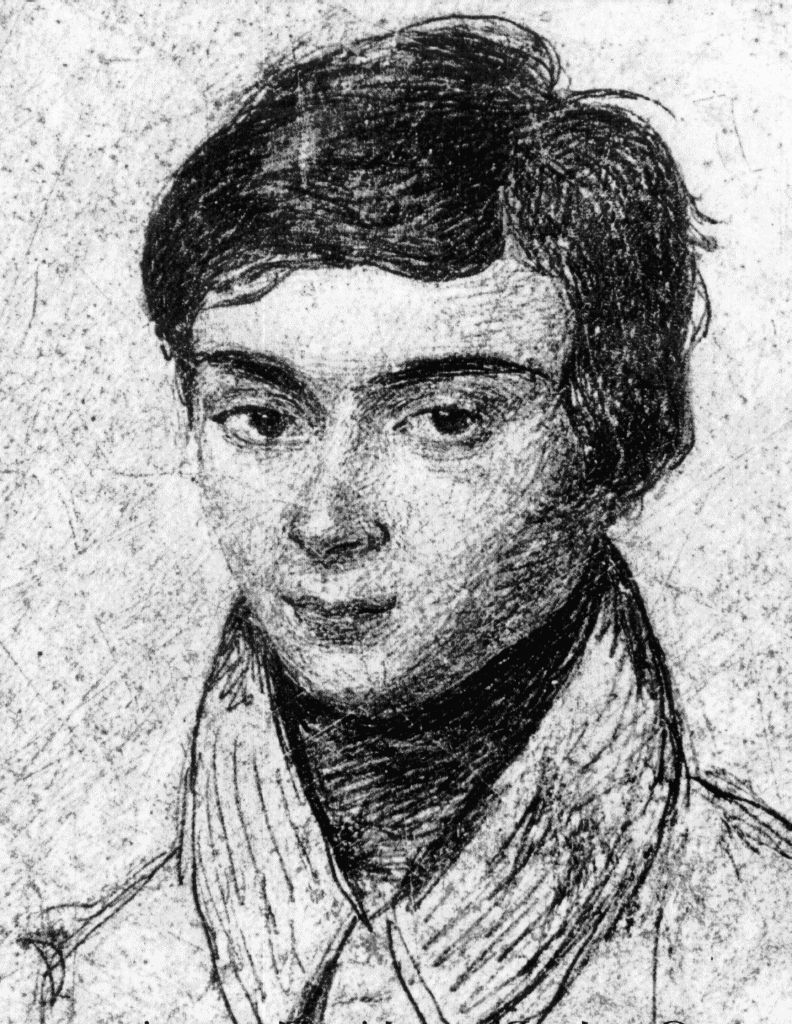
\includegraphics[width=0.7\linewidth]{Images/Evariste_galois}
				\caption{\tiny{Evariste Galois (25/10/1811 $–$ 31/5/1832) was a French mathematician born in Bourg-la-Reine. While still in his teens, he was able to determine a necessary and sufficient condition for a polynomial to be solvable by radicals.}}
			\end{figure}
		\end{column}
		\begin{column}{0.6 \textwidth}
			\begin{block}{Galois Theory}
				\footnotesize{
				Galois theory provides a answer to the question why there is no formula for the roots of a fifth (or higher) degree polynomial equation in terms of the coefficients of the polynomial, using only the usual algebraic operations (addition, subtraction, multiplication, division) and application of radicals (square roots, cube roots, etc). It also explains why it is possible to solve equations of degree four or lower in the above manner, and why their solutions take the form that they do.}
			\end{block}
		\end{column}
	\end{columns}

\end{frame}
\begin{frame}
	\begin{example}
		
		\begin{itemize}
			\small{
			\item Homogeneous recurrence relations: $y[k+2]-5y[k+1]+6y[k] = 0$
			\item Initial value: $y[0] =1$, $y[1] = 1$
			\item Characteristic polynomial: $r^2-5r+6=0$
			\item Roots: 2 and 3
			\item General solution: $c_1 2^k + c_2 3^k$
			\item Using the initial values: 
			\begin{center}
				$
				\begin{Bmatrix}
					1 = c_1 + c_2\\
					1 = 2c_1 + 3c_2\\
				\end{Bmatrix}
				$\\
					$
					\begin{Bmatrix}
					2 = c_1 \\
					-1 = c_2\\
					\end{Bmatrix}
					$\\
			\end{center}
			\item Result: $y[k] = 2^{k+1} - 3^{k}$}
		\end{itemize}
	\end{example}
\end{frame}
\begin{frame}
\frametitle{Example: Fibonacci sequence}
\begin{columns}
	\begin{column}{0.35\linewidth}
		
\begin{figure}
\centering
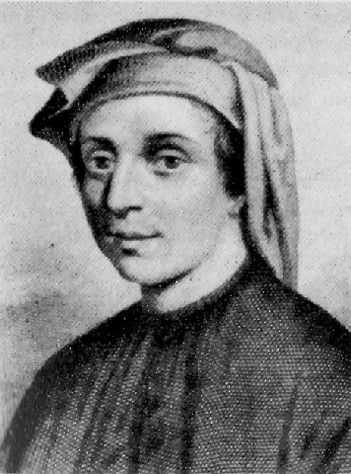
\includegraphics[height=0.5\textheight]{Images/discrete_time_systems_7}
\caption{\tiny{Leonardo Bonacci (c. 1170 $–$ c. 1250) known as Fibonacci was an Italian mathematician, considered to be "the most talented Western mathematician of the Middle Ages".}}

\end{figure}
	\end{column}
	\begin{column}{0.65\linewidth}
\begin{figure}
\centering
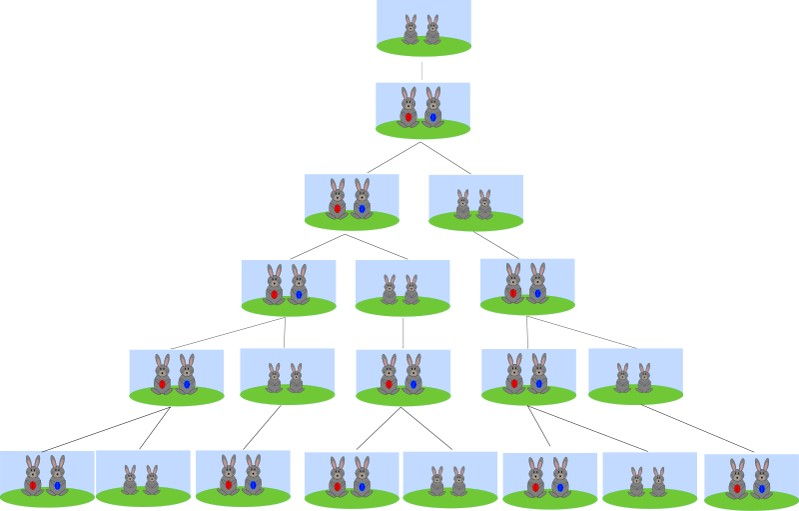
\includegraphics[width=0.9\linewidth]{Images/discrete_time_systems_8}
\caption{Fibonacci sequence}
\end{figure}
	\end{column}
\end{columns}
\end{frame}
\begin{frame}

	\frametitle{Example: Fibonacci sequence}
	\begin{example}
		\begin{itemize}
			
			\footnotesize{
			\setlength\itemsep{0em}
			\item Homogeneous recurrence relations: \\ $y[k+2] = y[k+1] + y[k]$
			\item Initial value: $y[0]=1, y[1]= 1$
			\item Characteristic polynomial: $r^2 - r - 1=0$ 
			\item Roots: $\frac{1+\sqrt{5}}{2}$ and $\frac{1-\sqrt{5}}{2}$
			\item General solution: $y[k] = c_1(\frac{1+\sqrt{5}}{2}) + c_2(\frac{1-\sqrt{5}}{2})$
			\item Initial values: 
			\begin{center}
				$
				\begin{Bmatrix}
				c_1+ c_2 = 1\\
				c_1 \frac{1+\sqrt{5}}{2} + c_2 \frac{1-\sqrt{5}}{2} = 1  \\
				\end{Bmatrix}
				$\\
				$
				\begin{Bmatrix}
				c_1 = \frac{5+\sqrt{5}}{10}  \\
				c_2 = \frac{5-\sqrt{5}}{10}
				\end{Bmatrix}
				$\\
			\end{center}
			\item Result: $y[k] =  (\frac{5+\sqrt{5}}{10})(\frac{1+\sqrt{5}}{2})^{k} +(\frac{5-\sqrt{5}}{10}) (\frac{1-\sqrt{5}}{2})^{k}$}
		\end{itemize}
	\end{example}
\end{frame}
\begin{frame}
	\frametitle{Multiple roots and complex roots}
	\begin{block}{Multiple roots}
		\scriptsize{For a multiple root $r_i$ with multiplicity m add $r_i^k$,$kr_i^k$,\dots,$k^{m-1}r_i^{k}$}
	\end{block}
	\begin{block}{Complex roots}
		\scriptsize{
		Complex roots will result in oscillating behaviour.
		If the difference equations and initial conditions are both real the complex roots can only be present in conjugate pairs, the constants will also be in conjugate pairs.
		\begin{center}
				$ r_i = Re^{j\phi}$ \quad	$r_{i+1} = Re^{-j\phi}$\\
				$c_i = R_0e^{j\phi_0}$ \quad	 $c_{i+1} = R_0e^{-j\phi_0}$\\
				$c_ir_i^k+c_{i+1}r_{i+1}^k = R_0Re^{jk\phi+j\phi_0} +  R_0Re^{-(jk\phi+j\phi_0)} $\\
				This can be converted into a cosine and sine using Eulers formula:	
				$y[k] = R_0R\big(\cos(k\phi+\phi_0) + \sin(k\phi+\phi_0) \big) + R_0R\big(\cos(k\phi+\phi_0) - \sin(k\phi+\phi_0) \big)$ \\
						 $= 2R_0R\big(\cos(k\phi+\phi_0)\big)$			
		\end{center}}
	\end{block}
\end{frame}
\begin{frame}
	\frametitle{Eulers formula}
	\begin{theorem}
		$e^{j\phi} = \cos(\phi) + \sin(\phi)j$
	\end{theorem}
	\begin{proof}
		Using power series:
		\begin{equation*}
				\begin{split}
				e^{\phi j} &= 1 + jx-\frac{x^{2}}{2!} - \frac{jx^{3}}{3!} + \frac{x^{4}}{4!} + \frac{jx^{5}}{5!} + \dots\\
				& = \bigg(1-\frac{x^{2}}{2!}+ \frac{x^{4}}{4!} + \dots\bigg)+\bigg(x - \frac{x^{3}}{3!} + \frac{x^{5}}{5!}+\dots\bigg)j\\
				&= \cos(\phi) + \sin(\phi j)
				\end{split}	
		\end{equation*}	
	\end{proof}
\end{frame}
\begin{frame}
	\begin{columns}
		\begin{column}{0.4\linewidth}
			\begin{figure}
			\centering
			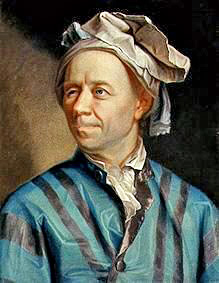
\includegraphics[width=0.7\linewidth]{Images/Leonhard_Euler}

			\end{figure}
		\end{column}
		\begin{column}{0.6\linewidth}
			Leonhard Euler (15/4/1707–18/9/1783) was a pioneering Swiss mathematician and physicist. He made important discoveries in fields as diverse as infinitesimal calculus and graph theory. He also introduced much of the modern mathematical terminology and notation, particularly for mathematical analysis, such as the notion of a mathematical function.
		\end{column}
	\end{columns}
\end{frame}
\begin{frame}
	\frametitle{Non-homogeneous difference equations}
	\begin{definition}
		\begin{center}
			$\sum\limits_{i=0}^n a_iy[k+i] = \sum\limits_{i=0}^n b_iu[k+i]$\\
		\end{center}
	 	A linear combination of inputs results in the same linear combination of the outputs resulting from each input individually.
	\end{definition}
	\begin{block}{Solution}
		The equation can thus be solved for each input individually and the results added together afterwards.
			
		The resulting particular solutions can then be added to the general form of the homogeneous solution.
	\end{block}
\end{frame}
\begin{frame}
	\frametitle{Particular solutions to difference equations}
	\begin{tabular}{|c|c|}
		\hline Input $u[k]$ & Suggested solution $y[k]$  \\ 
		\hline $k$ & $\alpha_1k+\alpha_0 $\\ 
		\hline $k^{n}$ & $\sum\limits_{i=0}^{n}\alpha_{i}k^{i}$ \\ 
		\hline $a^{k}$&  $\alpha a^{k}$\\ 
		\hline $k^{n}a^{k}$ & $(\sum\limits_{i=0}^{n}\alpha_{i}k^{i})a^{k}$  \\ 
		\hline $cos(k\phi)$ & $\alpha cos(k\phi + \phi_0)$\\ 
		\hline $a^{k}cos(k\phi)$ & $\alpha a^{k} cos(k\phi + \phi_0)$  \\ 
		\hline  $k^{n}a^{k}cos(k\phi)$&  $(\sum\limits_{i=0}^{n}\alpha_{i}k^{i}\alpha a^{k} cos(k\phi + \phi_0)$ \\ 
		\hline 
	\end{tabular} 
\end{frame}
\begin{frame}
	\frametitle{Example}
	\begin{example}
		\begin{itemize}
			\setlength\itemsep{0em}
			\small{
			\item Difference equation : $y[k+2] - 5y[k+1]+6y[k]=(-1)^k$
			\item Initial value:  $y[1] = \frac{1}{4}, y[0] = \frac{1}{12}$
			\item Homogeneous difference equation: $y[k+2] - 5y[k+1]+6y[k] = 0$
			\item Characteristic polynomial: $r^2-5r+6 = 0$
			\item Homogeneous solution: $y_{hom}[k] = c_{1}2^{k} + c_{2}3^{k}$
			\item Particular solution: $y_{par}[k] = \alpha(-1)^k$
			\item Substitution: $\alpha(-1)^{k+2}-5\alpha(-1)^{k+1}+6\alpha(-1)^k = (-1)^k$
			\item $\alpha = \frac{1}{12}$
			\item General solution: $y[k] = c_{1}2^{k}+c_{2}3^{k}+\frac{1}{12}(-1)^{k}$
			\item Using the initial values: $c_1 = -\frac{1}{3}, c_{2} = \frac{1}{3}$
			\item Result:  $y[k]= -\frac{1}{3}2^{k}+\frac{1}{3}3^{k}+\frac{1}{12}(-1)^{k}$}
		\end{itemize}
	\end{example}

\end{frame}
\section{Impulse response and convolution}
\begin{frame}
	\frametitle{Impulse response}
	
	\begin{definition}
		\footnotesize{
		$\delta[k]=
		\begin{cases} 
			1 & \text{if } k = 0 \\ 
			0 & \mbox{otherwise}  
		\end{cases}$}
	\end{definition}
	\vspace{-1em}
		\begin{figure}
			\centering
			\includegraphics[width=0.45\linewidth]{Images/Discrete_time_eps_8.eps}
		\end{figure}
		\vspace{-1em}
\begin{theorem}
	\scriptsize{
	You can decompose any signal as follows:\\
	$f[k]=\sum\limits_{i=-\infty}^{i=\infty}\delta[k-i]f[i] = \delta[k] \ast f[k]$}
\end{theorem}
\end{frame}
\begin{frame}
	\frametitle{Convolution}
	\begin{definition}
		$w[k]=u[k]\ast v[k] = \sum\limits_{i=-\infty}^{\infty} u[i]v[k-i]$
	\end{definition}
	\begin{block}{Solve}
		\begin{enumerate}
			\item Flip v[i] around vertical axis(v[-i]).
			\item Slide to the right over k steps(v[k-i]).
			\item Multiply $u[i]$ and $v[k-i]$
			\item Sum all the values.
		\end{enumerate}
	\end{block}
\end{frame}
\begin{frame}
	\frametitle{Convolution theorem }
	\begin{theorem}
		$y[k] = u[k] \ast h[k]$
	\end{theorem}
	\begin{proof}
		\begin{center}
				$ \delta[k] \rightarrow h[k]$\\
				$ \delta[k+i] \rightarrow h[k+i]$\\
				$ u[k] = \sum\limits_{i=-\infty}^{i=\infty}\delta[k-i]u[i] \rightarrow \sum\limits_{i=-\infty}^{i=\infty}h[k-i]u[i]$\\
				$u[k] \rightarrow u[k] \ast h[k] = y[k] $
		\end{center}
	\end{proof}
\end{frame}
\begin{frame}
	\begin{figure}
\centering
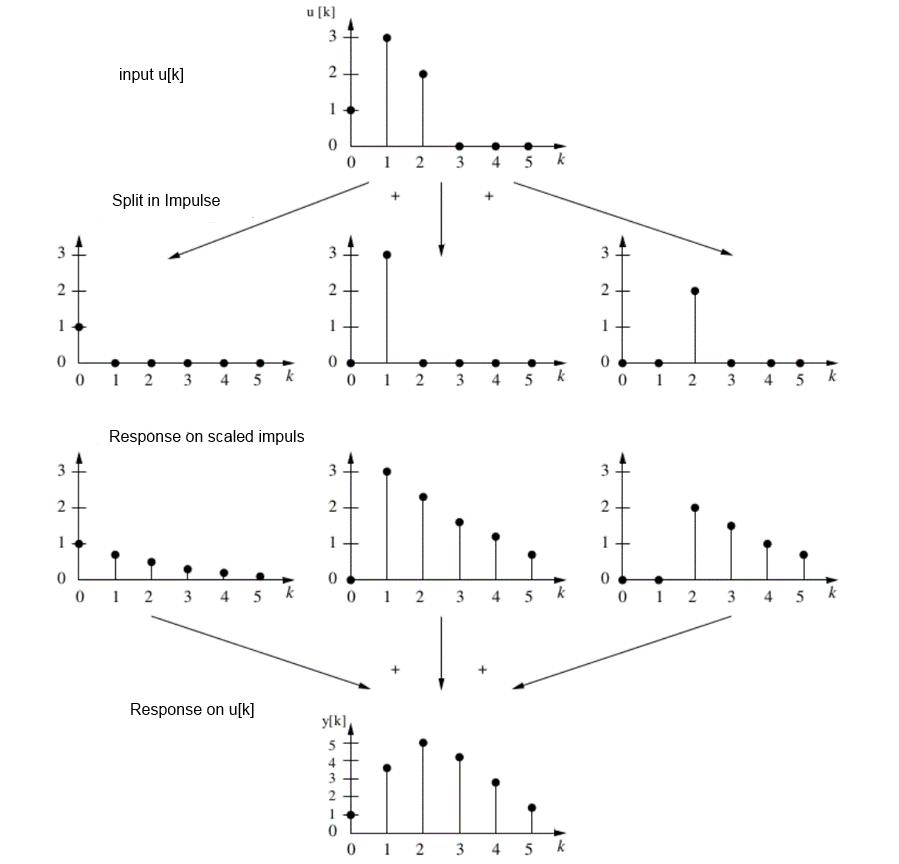
\includegraphics[height=0.9\textheight]{Images/discrete_time_systems_20}

\end{figure}

\end{frame}
\begin{frame}
	\frametitle{Impulse response}
	\begin{definition}[Impulse response]
		The impulse response of a dynamic system is  the output when the input is a unit-impulse.
	\end{definition}
	\begin{block}{Impulse response}
		$h[k] = \begin{cases}
			0  & \text{if } k <  0 \\
			D & \text{if } k= 0 \\ 
			CA^{k-1}B & \text{if } k> 0 
		\end{cases}$
	\end{block}
\end{frame}
\begin{frame}
	\frametitle{Examples of Dirac-delta’s}
	Popping balloons for acoustic measurements
	\begin{figure}
		\centering
		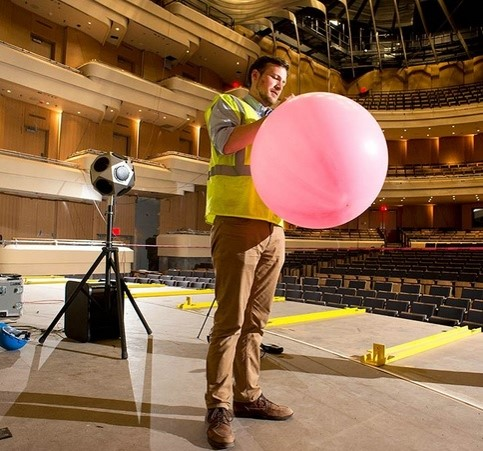
\includegraphics[height=0.7\textheight]{Images/discrete_time_systems_9}
	\end{figure}

\end{frame}
\begin{frame}
	\frametitle{Example: Leontief model of a planned economy}
	\begin{columns}
		\begin{column}{0.6 \textwidth}
			\begin{itemize}
					\item Won the Nobel prize in 1973
					\item A simple model that assigns values to different sectors
					\item For simplicity we choose a planned economy. But today governments all over the world are using similar models to model their economy.
			\end{itemize}
		\end{column}
		\begin{column}{0.4 \textwidth}
			
		\begin{figure}
			\centering
			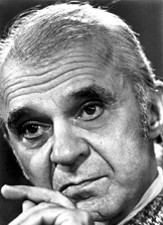
\includegraphics[width=0.8\linewidth]{Images/discrete_time_systems_10}	
			\end{figure}
		\end{column}
	\end{columns}

\end{frame}
\begin{frame}
	\frametitle{Example: Leontief model of a planned economy}
	Leontief divided the economy in sectors who buy from each other.\\
	The optimal production of some sector this month depends on the demand (external and internal) of the following month. So the system is non causal.\\
	\begin{center}
		\begin{align*}
			x[k-1] &= A x[k] + B u[k]\\
			y[k] &= I x[k]
		\end{align*}
	\end{center}	
\end{frame}

\section{Z-transform}
\begin{frame}{Z-transform}
	\begin{definition}
		\begin{itemize}
			\item Discrete equivalent to the Laplace-transform
			\item Converts time-dependent descriptions of systems to the time-independent Z-domain.
			\item Simplifies many calculations:
			\begin{itemize}
				\item 	Convolution theorem $\rightarrow$ convolution becomes multiplication
				\item Linear difference equations become simple algebraic expressions
				\item \dots
			\end{itemize}
		\end{itemize}
	\end{definition}
\end{frame}
\begin{frame}
		\begin{figure}
			\Wider{
			\centering
			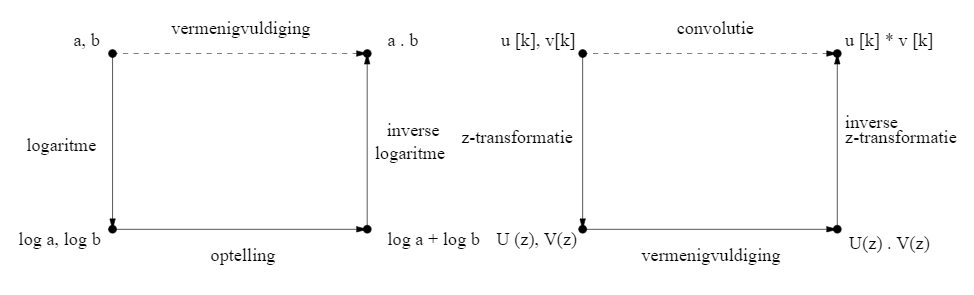
\includegraphics[width=1\linewidth]{Images/discrete_time_systems_21}}
		\end{figure}
		
\end{frame}
\begin{frame}
	\frametitle{Z-transform}
	\begin{block}{2 forms}
			\begin{itemize}
				
				\item Bilateral:
				Requires knowledge of x for all values of k, including negative values.
				Can be used for non-causal systems $X(z) = \sum\limits_{k=-\infty}^{\infty} x[k]z^{-k}$
				\item 	Unilateral:
				Only requires knowledge of x for positive values of k.
				Can only be used for causal systems without loss of information $X(z) = \sum\limits_{k=0}^{\infty} x[k]z^{-k}$
			\end{itemize}
	\end{block}


\end{frame}
\begin{frame}
	\frametitle{Z-transform}
		\begin{example}
			\begin{center}
				
				$x[k] = \begin{Bmatrix}
				1 & - 1 & 0 & 2 & 4\\
				&     &   & \uparrow & \\
				\end{Bmatrix}$
			\end{center}
			\begin{center}
				$X(z) = \sum\limits_{k=-3}^{1}x[k]z^{-k} = z^3 -z^2 +2 + 4z^{-1}$
			\end{center}
		\end{example}	
\end{frame}
\begin{frame}
	\frametitle{Properties Unilateral Z-transform}
	\small{
		\begin{tabular}{|c|c|c|}
			\hline  Property & Time Domain & Z-domain  \\ 
			\hline  Linearity & $af_1[n]+bf_2[n] + \dots  $& $aF_1(Z)+bF_2(Z)+\dots$ \\ 
			\hline  Right Shift(m$>$0)& $f[k-m]$  &$z^{-m}F(Z)$  \\ 
			\hline  Left Shift (m$>$0)& $f[k+m] $  & $ z^m\bigg(F(z)-\sum\limits_{i=0}^{m-1}f[i]z^{-i} \bigg)$ \\ 
			\hline  Convolution & $f[k]\ast g[k] $  & $F(z)G(z) $ \\ 
			\hline  Multiplication by $a^{k}$ & $a^{k}f[k]$  & $F(a^{-1}z)$  \\ 
			\hline  Summation in time& $\sum\limits_{i=0}^{k}f[i]$  & $\frac{z}{z-1}F(Z) $\\ 
			\hline  Differentiation in z& $k^mf[k]$ & $\big(-z \frac{d}{d}\big)^{m} F(z)$ \\ 
			\hline  Periodic Sequence & $f[k] = f[k+N]$  & $F(z) = \frac{z^N}{z^{N-1}}\sum\limits_{k=0}^{N-1}f[k]z^{-1}$  \\ 
			\hline  Initial Value& f[0] &$ \lim_{\mid z \mid \to \infty} F(z) $  \\ 
			\hline  Final value & $f[\infty] $ & $\lim_{z \to 1} (z-1)F(z) $ \\ 
			\hline 
		\end{tabular} }
\end{frame}
\begin{frame}
	\frametitle{List of common Z-transform pairs}
	\begin{figure}
\centering
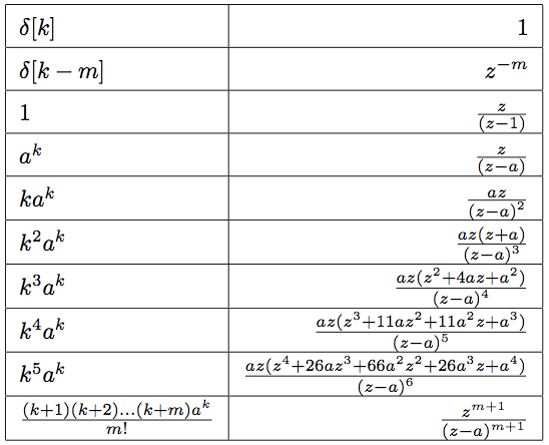
\includegraphics[height=0.8\textheight]{Images/discrete_time_systems_22}

\label{fig:discrete_time_systems_22}
\end{figure}

	
\end{frame}
\begin{frame}
	\frametitle{List of common Z-transform pairs}
	\begin{figure}
\centering
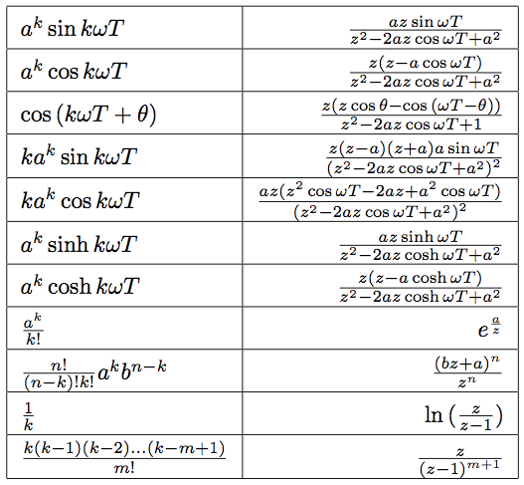
\includegraphics[height=0.8\textheight]{Images/discrete_time_systems_23}
\label{fig:discrete_time_systems_23}
\end{figure}

\end{frame}
\begin{frame}
	\frametitle{Region of convergence}
	\begin{alertblock}{Z-transform is not unique}
		Two different signals could have the same Z-transform over a different region of convergence.
	\end{alertblock}
	\begin{definition}
		The region of convergence is the set of complex numbers z for which:
		\vspace{-2em}
		\begin{center}
			$\sum\limits_{k=-\infty}^{\infty} \mid x[k]z^{-k} \mid < \infty$
		\end{center}
		
	\end{definition}
	
	
\end{frame}
\begin{frame}
		\begin{itemize}
			\item We will look at convergence separately for positive and negative k, splitting the convergence criterion in 2:
			\begin{center}
				$k<0: \mid x[k] \mid \leq M_{-}R_{-}^{k}$\\
				$k\geq 0: \mid x[k] \mid \leq M_{+}R_{+}^{k} $
			\end{center}
			\item Using $z = r e^{j\theta}$ with R+ as small as possible and R- as large as possible we get:
			\vspace{-2em}
			\begin{center}
				\begin{align*}
				\sum\limits_{k=-\infty}^{\infty} \mid x[k]z^{-k} \mid &= \sum\limits_{k=-\infty}^{\infty} \mid x[k] \mid r^{-k} \\
				&= \sum\limits_{k=1}^{\infty} \mid x[-k] \mid r^{k} + \sum\limits_{k=0}^{\infty} \mid x[k] \mid r^{-k} \\
				&\leq M_{-} \sum\limits_{k=1}^{\infty} (R_{-}^{-1}r)^{k} + M_{+} \sum\limits_{k= 0}^{\infty}(R_{+}r^{-1})^{k}
				\end{align*}
			\end{center}
		\end{itemize}
\end{frame}
\begin{frame}
\frametitle{Region of convergence}
The sums are finite if $R_{-}^{-1}r < 1$ and $R_{+}r^{-1} < 1$
Region of convergence: $R_{+} < R_{-}$
R+< R-: Ring
R-< R+: No ROC
Causal system, for negative k:
$x[k] = 0 \Rightarrow R_{-} = + \infty$
cannot contain any poles of the system
ROC of a stable system always contains
the unit circle.
\begin{figure}
\centering
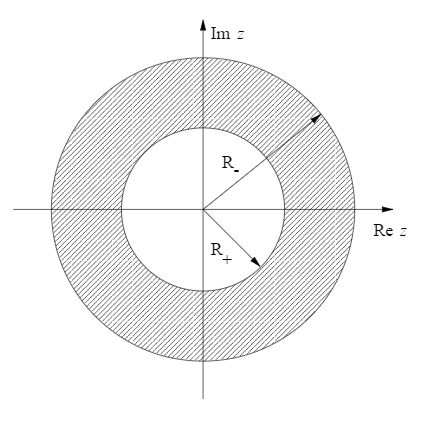
\includegraphics[height=0.5\textheight]{Images/discrete_time_systems_24}
\label{fig:discrete_time_systems_24}
\end{figure}

\end{frame}
\begin{frame}
	\frametitle{Inverse Z-transform}
	\begin{block}{Inverse Z-transform}
		\begin{enumerate}
			\item Split the function into partial fractions
			\item Use the table to transform each partial fraction individually to the time domain
		\end{enumerate}
	\end{block}
	
\end{frame}
\begin{frame}
	\begin{block}{Partial fraction decomposition}
		\begin{enumerate}
			\item Factorizing the denominator
			\item If all poles(zeros of the denominator) have multiplicity 1:
			\vspace{-2 em}

				\begin{align*}
				F(z) &= \frac{\sum\limits_{i=0}^{n} b_i z^{i}}{a_n(z-p_1)(z-p_2) \dots (z-p_n)}\\
				&= \alpha_0 + \alpha_1 \bigg(\frac{z}{z-p_1}\bigg)  + \dots + \alpha_n \bigg(\frac{z}{z-p_n}\bigg)
				\end{align*}
			
			\item The coefficients can be calculated by:\\
			\begin{center}
				$\alpha_0 = F(0)$ \quad		$\alpha_i = \bigg[\frac{z-p_i}{z} F(z)\bigg]_{z=p_i}$
			\end{center}
			\newcounter{enumTemp}
			\setcounter{enumTemp}{\theenumi}
		\end{enumerate}
	\end{block}
\end{frame}
\begin{frame}
	\frametitle{Inverse Z-transform}
	\begin{block}{Partial fraction decomposition}
			\begin{enumerate}
				\setcounter{enumi}{\theenumTemp}
				\footnotesize{
				\item If there are poles with multiplicity higher than 1:
				\vspace{-1.25em}
					\begin{align*}
						F(z) & = \frac{\sum\limits_{i=0}^{n} b_i z^{i}}{a_n(z-p_1)^{n_1}(z-p_2)^{n_2} \dots}\\
						& = \alpha_0 + \alpha_1\bigg(\frac{z}{z-p_1}\bigg) + \alpha_2\bigg(\frac{z}{z-p_1}\bigg)^{2} + \dots + \alpha_{n_1}\bigg(\frac{z}{z-p_1}\bigg)^{n_1} \\
						& + \beta_1 \bigg(\frac{z}{z-p_2}\bigg) + \beta_2 \bigg(\frac{z}{z-p_2}\bigg)^{2} + \dots \beta_{n_2} \bigg(\frac{z}{z-p_2}\bigg)^{n_2}
					\end{align*}
					\item Where the highest coefficient for each pole can be calculated by:
					\begin{center}
						$ \alpha_0 = F(0)$ 		$\alpha_1 = \Bigg[\bigg(\frac{z-p_1}{z}\bigg)^{n_1}F(z)\Bigg]_{z=p_1}$ 	 $\beta_1 = \Bigg[\bigg(\frac{z-p_2}{z}\bigg)^{n_2}F(z)\Bigg]_{z=p_2}$
					\end{center}}
					\newcounter{enumTmp}
					\setcounter{enumTmp}{\theenumi}
				\end{enumerate}
	\end{block}

\end{frame}
\begin{frame}
	\frametitle{Inverse Z-transform}
	\begin{block}{Partial fraction decomposition}
			\begin{enumerate}
				\setcounter{enumi}{\theenumTmp}
				\item Any remaining coefficients can be found by evaluating the equation for a number of values of z.
			\end{enumerate}
				\begin{tabular}{|c|c|}
					\hline $F(z)$ & $f[k]$ \\
					\hline $1$ & $\delta[k]$ \\
					\hline $\frac{z}{z-a}$ & $ a^{k}$ \\
					\hline $\frac{z^{m+1}}{(z-a)^{m+1}}$ & $\frac{(k+1)(k+2)+ \dots (k+m)a^{k}}{m!}$ \\ 
					\hline 
				\end{tabular} 
	\end{block}

\end{frame}
\begin{frame}
	\frametitle{Inverse Z-transform}
	\begin{example}
		\footnotesize{
		\begin{center}
			$F(z) = \frac{z^3 + 2 z^2 + z +1}{z^3-z^2-8z +12}$
		\end{center}
		\vspace{-1.5 em}
		\begin{itemize}
			\item The denominator has a zero in 2 (m=2) and -3
			\item Partial fraction decomposition:
			\begin{center}
				$\alpha_0 +\alpha_1 \bigg(\frac{z}{z-2}\bigg)+ \alpha_2 \bigg(\frac{z}{z-2}\bigg)^{2} + \beta_1 \bigg(\frac{z}{z+3}\bigg)$
			\end{center}
			
			\item \begin{center}
				$\alpha_0 = F(0) = \frac{1}{12} $ \\
				$\alpha_2 =\Bigg[\frac{F(z)(z-2)^{2}}{z^2}\Bigg]_{z=2} = \Bigg[\frac{z^3+2z+z+1}{z^2(z+3)}\Bigg]_{z=2} = \frac{19}{20}$\\
				$\beta_1 =\Bigg[\frac{F(z)(z+3)}{z}\Bigg]_{z=-3} = \Bigg[\frac{z^3+2z+z+1}{z(z-2)^2}\Bigg]_{z=-3} = \frac{11}{75}$ 
			\end{center}
		
		\end{itemize}}
	\end{example}
\end{frame}
\begin{frame}
	\begin{example}
		\begin{itemize}
				\item By evaluating the function for z=1:\\
				$\frac{5}{4} = \alpha_0 - \alpha_1 + \alpha_2 + \beta/4$\\
				$\alpha_1 = -9/50$
				\item Result : $F(z) = \frac{1}{12} - \frac{9}{50} \frac{z}{z-2} + \frac{19}{20} \frac{z^2}{(z-2)^2} + \frac{11}{75} \frac{z}{z+3}$
				\item Inverse Z-transform: $f[k] = \delta[k]/12 + 2^k k \frac{19}{20}
				+ 2^k \frac{77}{100} + (-3)^k \frac{11}{75}$
		\end{itemize}
	\end{example}
\end{frame}
\begin{frame}
	\frametitle{Inverse Z-transform}
	Another technique for calculating the inverse Z-transform is direct division.\\
	The numerator of the transfer function is divided by the denominator via long division.
	\begin{figure}
		\centering
		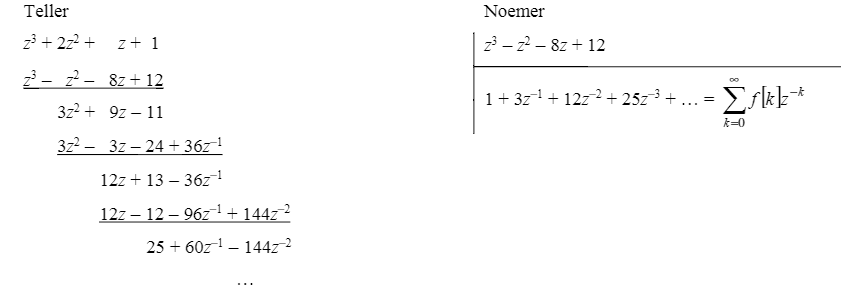
\includegraphics[width=0.9\linewidth]{Images/discrete_time_systems_25}
		\label{fig:discrete_time_systems_25}
	\end{figure}
	
\end{frame}
\begin{frame}
	\frametitle{Solving difference equations with the Z-transform}
	A system is described by a difference equation of the following form:
	\begin{center}
		$\sum\limits_{i=0}^n a_iy[k+i] = \sum\limits_{i=0}^n b_iu[k+i]$
	\end{center}
	After the Z-transform:
	\begin{center}
		$a_0 Y(z) + \sum\limits_{i=1}^{n} a_i z^i \Bigg[Y(z)-\sum\limits_{j=0}^{i-1}y[j]z^{-j}\Bigg] = b_0U(z)+\sum\limits_{i=1}^{n} b_i z_i \Bigg[U(z)-\sum\limits_{j=0}^{i-1}u[j]z^{-j}\Bigg]$
	\end{center}

\end{frame}
\begin{frame}
		\frametitle{Solving difference equations with the Z-transform}
		Rearranged:
		\begin{center}
			$Y(z) = \frac{\sum\limits_{i=1}^{n} b_i z^i}{\sum\limits_{i=1}^{n} a_i z^i} U(z) - \frac{\sum\limits_{i=1}^{n} b_i z^i \Bigg[\sum\limits_{j=0}^{i-1}u[j]z^{-j}\Bigg]-\sum\limits_{i=1}^{n} a_i z^i \Bigg[\sum\limits_{j=0}^{i-1}y[j]z^{-j}\Bigg]}{\sum\limits_{i=1}^{n} a_i z^i}$
		\end{center}
\end{frame}
\begin{frame}
	\frametitle{Solving difference equations with the Z-transform}
	We'll apply the following transformation of the double summations:\\
	$ \sum\limits_{i=1}^{n} b_i z^i \sum\limits_{j=0}^{i-1}u[j]z^{-j} = \sum\limits_{s=1}^{n}\sum\limits_{j=0}^{n-s}b_{s+j}u[j]	z^{s}$
	\begin{figure}
	\centering
	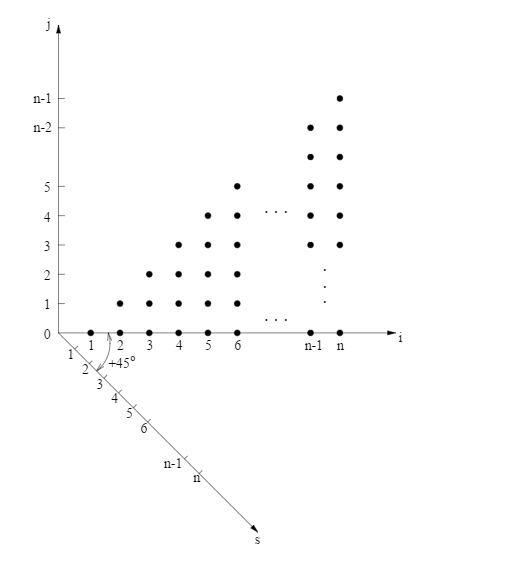
\includegraphics[height = 0.6\textheight]{Images/discrete_time_systems_26}
	\label{fig:discrete_time_systems_26}
	\end{figure}

\end{frame}
\begin{frame}
	\frametitle{Solving difference equations with the Z-transform}
	\footnotesize{The final simplified result is:\\
		$Y(z) = \frac{\sum\limits_{i=1}^{n} b_i z^i}{\sum\limits_{i=1}^{n} a_i z^i} U(z) + \frac{\sum\limits_{s=1}^{n}\Bigg(\sum\limits_{j=0}^{n-s}a_{s+j}y[j]-\sum\limits_{j=0}^{n-s}b_{s+j}u[j]\Bigg)	z^{s}}{\sum\limits_{i=1}^{n} a_i z^{i}}$\\
		With this result it is easy to find the resulting output from a given input or vice-versa given a difference equation.\\
		Right-hand fraction = output resulting from initial conditions: will vanish with time = transient behaviour\\
		Left-hand fraction = output resulting from input: will remain = steady state response. \\
		$ H(z) = \frac{\sum\limits_{i=1}^{n} b_i z_i}{\sum\limits_{i=1}^{n} a_i z_i}$ is the “transfer function” of the system. This is the z transform of $h[k]$ (the impulse response)}
		
\end{frame}
\begin{frame}
	\footnotesize{
	The transfer function can also be derived directly from the state space model of a system:\\
	\vspace{-1.5em}
	\begin{center}
		$x[k+1] = Ax[k] + Bu[k] $\\
		$y[k] = Cx[k]+Du[k]$
	\end{center}
	\vspace{-1.5em}
	The Z-transform gives:
	\begin{center}
		$z(X(z)-x[0]) = AX(z)+BU(z)$\\
		$Y(z) = CX(z)+DU(z)$
	\end{center}
	Rearranged to have X(z) in explicit form:
	\begin{center}
		$X(z) = (zI-A)^{-1}zx[0] + (zI-A)^{-1}BU(z) $\\
		$Y(z) = C(zI-A)^{-1}zx[0] + \bigg[C(zI-A)^{-1}B + D\bigg]U(z)$
	\end{center}
	If $x[0] = 0$ and $u[k] = \delta[k] (U(z)=1)$:\\
	$H(z) = C(zI-A)^{-1}B + D$\\
	$Y(z)=H(z)U(z)$}
\end{frame}
\begin{frame}
	\frametitle{Z-Transform}
	\begin{definition}
		A pole $p_i$ of the is system is a point in the complex z-plane where $H(p_i) = \pm \infty$ i.e. the denominator becomes zero.\\
		\begin{center}
			$\sum\limits_{i=0}^{n}a_iz^{i} = 0$
		\end{center}
	\end{definition}
	\begin{definition}
		A zero $n_i$ is a point where $H(n_i)=0$ i.e. the numerator becomes zero.\\
		\begin{center}
			$\sum\limits_{i=0}^{n}b_iz^{i} = 0$
		\end{center}
	\end{definition}
\end{frame}
\begin{frame}
	\frametitle{Link between eigenvalues and poles}
	\textbf{Are eigenvalues of A poles of H(z)?}\\
	\small{
	\begin{itemize}
			\item As z approaches an eigenvalue of A, $(zI-A)^{-1}$ is no longer defined.\\
			\item $C(zI-A)^{-1}B$	may still be defined depending on the values of C and B.
	\end{itemize}
}
	\begin{block}{Rule 1}
			An Eigenvalue of A will sometimes, but not always, be a pole of H(z).
	\end{block}
	\begin{definition}
		If every eigenvalue of A is also a pole of H(z) then a minimal number of internal states has been achieved.
	\end{definition}
	
	
\end{frame}
\begin{frame}
	\frametitle{Link between eigenvalues and poles}
	\textbf{Are poles of H(z) eigenvalues of A?}\\
	$H(z) = C(zI-A)^{-1}B + D$ \\
	B, C and D are matrices with properly defined values.
	If H(z) is undefined then $(zI-A)^{-1}$ must be the cause. So,
	z must be an eigenvalue of A
	\begin{block}{Rule 2}
		Poles of H(z) are always eigenvalues of A 
	\end{block}
\end{frame}
\begin{frame}
	\frametitle{Stability}
	\begin{itemize}
		\item Internal Stability
		\begin{itemize}
			\item All possible internal states return to zero after a finite time in the absence of an input.
			\item 	All eigenvalues of the matrix A are contained within the a circle of radius 1 around zero in the complex plane.
		\end{itemize}
		\item BIBO-Stability (Bounded-Input Bounded-Output)
		\begin{itemize}
			\item Every bounded input results in a bounded output
			\item All poles are contained within the a circle of radius 1 around zero in the complex plane
			\item BIBO-Stability follows from Internal Stability, but the inverse is not necessarily true.
		\end{itemize}
	\end{itemize}
\end{frame}
\begin{frame}
\begin{figure}
\centering
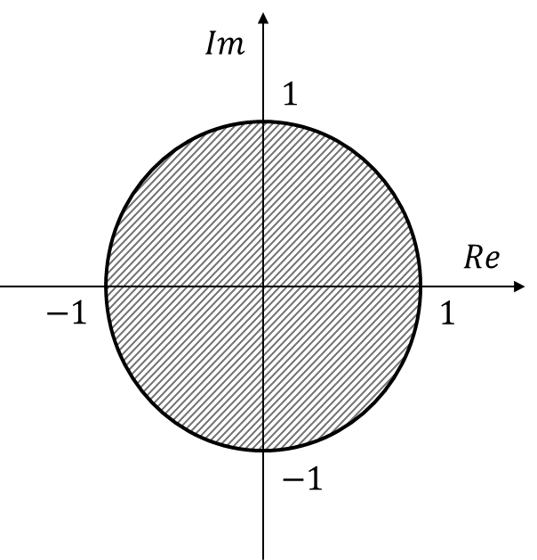
\includegraphics[height=0.7\textheight]{Images/discrete_time_systems_27}
\label{fig:discrete_time_systems_27}
\end{figure}
\end{frame}
\begin{frame}
	\frametitle{Can unstable systems exist?}
	According to the mathematical models we have discussed unstable systems need an infinite amount of energy.\\
	\textbf{What happens in the real world?}
	\begin{itemize}
		\item The system enters a state in which the current linear model is no longer valid (Non linear behaviour) .
		\item Smaller unaccounted effects become more prominent
		\item The system malfunctions and may cause damage to itself or its surroundings.
		\item Something else bad happens
	\end{itemize}
\end{frame}
\begin{frame}
	\frametitle{Stability}
	\begin{figure}
	\centering
	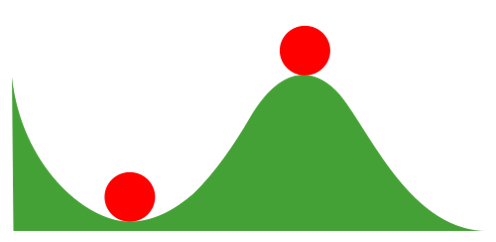
\includegraphics[width=0.7\linewidth]{Images/discrete_time_systems_29}
	\label{fig:discrete_time_systems_29}
	\end{figure}

\end{frame}
\begin{frame}
	\frametitle{Airplane stall}
	\begin{figure}
		\centering
		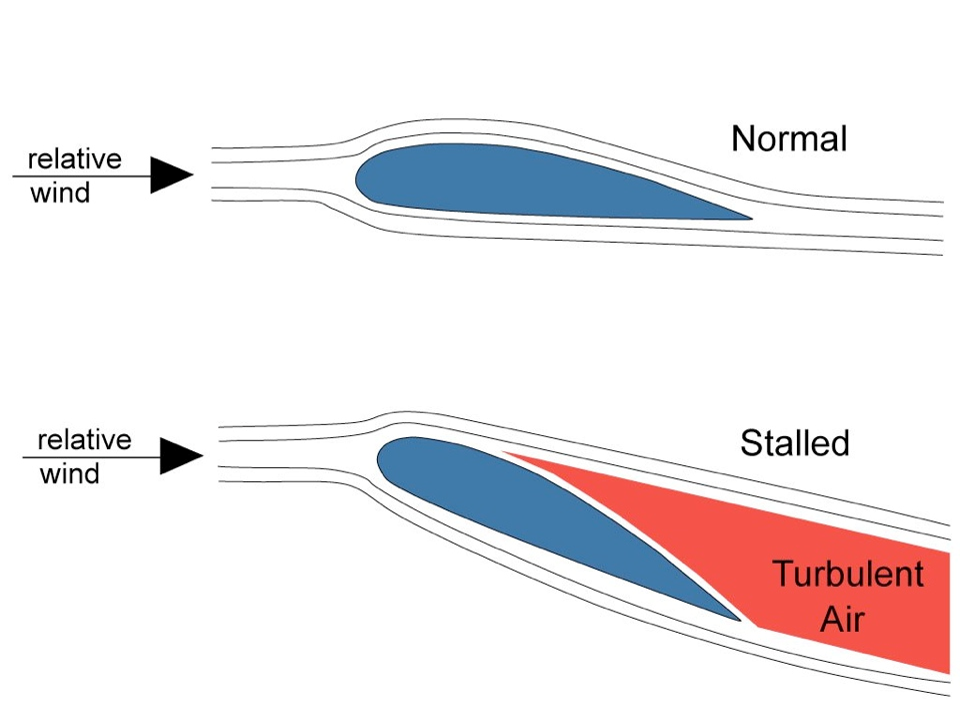
\includegraphics[height=0.7\textheight]{Images/discrete_time_systems_30}
		\label{fig:discrete_time_systems_30}
	\end{figure}
\end{frame}
\begin{frame}
	\begin{itemize}
		\item Airplanes generate lift using the Venturi effect.
		\item Faster moving air has a lower pressure.
		\item Eddy currents may be created due to a too slow airspeed or too sharp ascent.
		\item Turbulent airflow causes a loss of the lift generated by the Venturi effect.
		\item Without the necessary lift an air plane becomes an unstable system.
	\end{itemize}
\end{frame}
\begin{frame}
	\begin{columns}
		\begin{column}{0.6\textwidth}
			Buses and other tall vehicles have a tendency to roll when taking turns too quickly.
			A London bus is loaded with sandbags and must be able to lean  at an angle of at least $28^{\circ}$ while still returning all tires to the ground.
			Modern day car manufacturers have to pass multiple tests for stability while manoeuvring
		\end{column}
		\begin{column}{0.4\textwidth}
			\begin{figure}
				\centering
				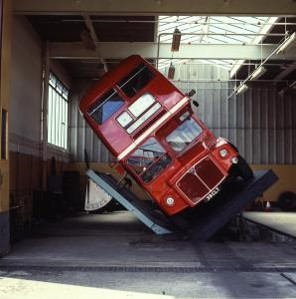
\includegraphics[width=0.8\linewidth]{Images/discrete_time_systems_32}
				\label{fig:discrete_time_systems_32}
			\end{figure}
		\end{column}
	\end{columns}
\end{frame}
\begin{frame}
	\frametitle{Steady state behavior via Z-transform}
	Starting from the previous result:\\
	$Y(z) = \frac{\sum\limits_{i=1}^{n} b_i z^i}{\sum\limits_{i=1}^{n} a_i z^i} U(z) + \frac{\sum\limits_{s=1}^{n}\Bigg(\sum\limits_{j=0}^{n-s}a_{s+j}y[j]-\sum\limits_{j=0}^{n-s}b_{s+j}u[j]\Bigg)z^{s}}{\sum\limits_{i=1}^{n}a_i z^i}$\\
	We wish to find the resulting output from the input:\\
	$ u[k] = \cos(k\alpha + \theta)$\\
	To simplify derivation, we use:\\
	$u[k] = e^{j(k\alpha + \theta)}$\\
	With Z-transform:	$U(z) = \frac{ze^{j\theta}}{z-e^{j\alpha}}$
	
\end{frame}
\begin{frame}
	\frametitle{Steady state behavior via Z-transform}
	Filling in U(z) and splitting into partial fractions:
	\begin{align*}
			Y(z) &= \frac{\sum\limits_{i=1}^{n} b_i z^i}{\sum\limits_{i=1}^{n} a_i z^i} \frac{ze^{j\theta}}{z-e^{j\alpha}} + \frac{\sum\limits_{s=1}^{n}\Bigg(\sum\limits_{j=0}^{n-s}a_{s+j}y[j]-\sum\limits_{j=0}^{n-s}b_{s+j}u[j]\Bigg)	z^{s}}{\sum\limits_{i=1}^{n} a_i z^{i}}\\
			& = \frac{cz}{z-e^{j\alpha}} + \frac{d_1z}{z-p_1} + \dots + \frac{d_nz}{z-p_n}+g\\
	\end{align*}
	Calculating the coefficient c:\\
	$c= \bigg[Y(z)\frac{z-e^{j\alpha}}{z}\bigg]_{z=e^{j\alpha}} = \bigg[H(z)e^{j\theta}\bigg]_{z=e^{j\alpha}} = H(e^{j\alpha})e^{j\theta}$\\

\end{frame}
\begin{frame}
	\frametitle{Steady state behavior via Z-transform}
	\small{
		After the inverse Z-transform:
		\begin{align*}			y[k]&=H(e^{j\alpha})e^{j(k\alpha+\theta)}+d_1p_1^k+\dots+d_np_n^{k}+g\delta[k]\\
		 &= \mid H(e^{j\alpha}) \mid e^{j(k\alpha+\theta+\angle H(e^{j\alpha}))} +d_1p_1^k+\dots+d_np_n^{k}+g\delta[k]
		\end{align*}
		
	Because of linearity we can ignore the imaginary component, leading to the result:\\
	$y[k] =  \underbrace{\mid H(e^{j\alpha}) \mid cos(k\alpha+\theta+\angle H(e^{j\alpha}))}_{\text{staedy state}} + \underbrace{Re(d_1p_1^k+\dots+d_np_n^{k}+g\delta[k])}_{\text{transient behavure}}$\\
	\begin{tabular}{|c|c|}
		\hline Input & Output \\ 
		\hline $cos(k\alpha + \theta)$ &  $\mid H(e^{j\alpha}) \mid cos(k\alpha+\theta+\angle H(e^{j\alpha}))$ \\ 
		\hline 
	\end{tabular} }
\end{frame}
\begin{frame}
	\frametitle{Steady state behavior via Z-transform}
	\begin{example}
		\begin{itemize}
			\item $u[k] = cos(3k+\pi) \Rightarrow \alpha = 3 \quad \theta = pi$
			\item $H(z) = \frac{z^2+4}{(z^2+6)(z-1)}$
			\item $H(e^{3j}) = 0.357e^{0.055j}$
			\item The resulting output has been reduced to a third in amplitude and has undergone a small phase shift. \\
			$ y[k] =0.357 \cos(3k+\pi + 0.055)$
			
		\end{itemize}
	\end{example}
\end{frame}
\begin{frame}
	\frametitle{Complex Eigenvalues }
	As with the roots to the characteristic equation in difference equations, complex and/or negative eigenvalues for A create oscillation.
	$\lVert\lambda\rVert < 1$: The oscillation will decrease in magnitude: stable
	$\lVert\lambda\rVert > 1$: The oscillation will increase in magnitude:  unstable
	$\lVert\lambda\rVert = 1$: The oscillation will maintain the same magnitude indefinitely:  unstable
	
	The smallest achievable period is 2 times the step time, for negative real eigenvalues.
	
\end{frame}
\begin{frame}
		\frametitle{Complex Eigenvalues }
		\begin{figure}
			\centering
			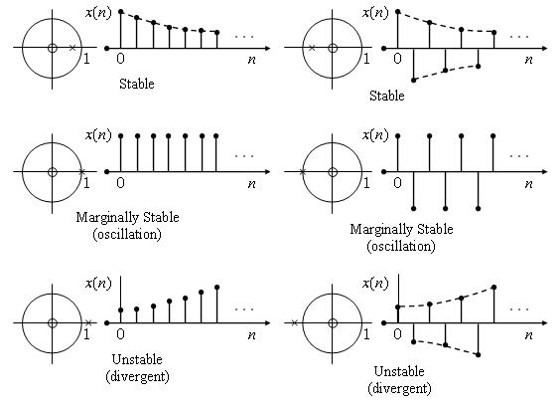
\includegraphics[width=0.7\linewidth]{Images/discrete_time_systems_33}
		\end{figure}
\end{frame}
\section{Observability and controllability}
\begin{frame}
	\frametitle{Observability and controllability}
	\begin{figure}
	\centering
	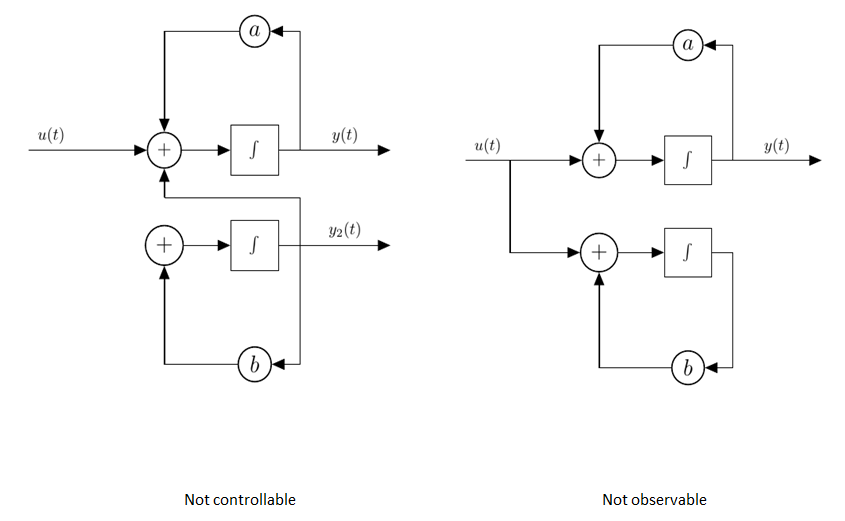
\includegraphics[width=0.7\linewidth]{Images/discrete_time_systems_34}
\end{figure}
\end{frame}
\begin{frame}
	\frametitle{Observability}
	\small{
	A system is observable if every initial state $x[0]$ can be determined from the observation of y[k].\\
	The state space model without inputs gives us:\\
	$x[k+1] = A x[k] $ \quad \quad				$y[k]=Cx[k]$\\
	Now we can determine a set of vector equations in $x[0]$\\
	$x[1] = A x[0],x[2]  = A^2x[0],\dots , x[n-1] = A^{n-1} x[0]$\\
	If the system has n internal states then n equations are needed:\\
	$y[0] =Cx[0],y[1]=Cx[1]=CAx[0],\dots, y[n-1] = C A^{n-1} x[0]$\\
	\[
	\begin{bmatrix}
		y[0]\\
		y[1]\\
		\vdots \\
		y[n-1]\\
	\end{bmatrix} = 
	\begin{bmatrix}
	C\\
	CA\\
	\vdots\\
	CA^{n-1}\\
	\end{bmatrix} \begin{bmatrix}
	x_1[0]\\
	x_2[0]\\
	\vdots\\
	x_n[0]\\
	\end{bmatrix}
	\]}
\end{frame}
\begin{frame}
	\frametitle{Observability}
	The system is observable if 
	\[	\begin{bmatrix}
		C\\
		CA\\
		\vdots\\
		CA^{n-1}\\
	\end{bmatrix} \] has rank n.
\end{frame}
\begin{frame}
	\frametitle{controllable}
	A system is controllable if it can be brought to a desired state using the inputs in a finite time.\\
	Again we start from the state space model:\\
	The following equations can be derived:\\
	$x[k+1] = A x[k] +Bu[k]$\\
	$x[1] = Ax[0]+Bu[0]$\\
	$x[2] = A^2 x[0] + ABu[0] + Bu[1]$\\
	$x[3] = A^3 x[0] + A^2Bu[0]+AB u[1] + Bu[2]$\\
	$ \hspace{3 em}\vdots$\\
	$x[n] = A^{n}x[0]+A^{n-1}Bu[0] + \dots + Bu[n-1]$
\end{frame}
\begin{frame}
	\frametitle{Controllability}
	This last equation can be rewritten as:
	$x[n] - A^{n}x[0] = \begin{bmatrix}
	B & AB & \dots & A^{n-1}B
	\end{bmatrix}$ $
	\begin{bmatrix}
	u[n-1]\\
	u[n-2]\\
	\vdots\\
	u[1]\\
	u[0]
	\end{bmatrix}
	 $	\\
	For a given x[0] and a desired x[n] the required inputs can be found by solving this system.
	$\begin{bmatrix}
		B & AB & \dots & A^{n-1}B
	\end{bmatrix}$ is called the controllability matrix of the system.
	A system is said to be controllable if the set of equations can be solved for a given x[0] and any desired x[n].
	This is the case if the controllability matrix has a rank n.
	
\end{frame}
\begin{frame}
	\frametitle{Detectability and Stabilizability}
	Observability and controllability are important terms in control theory.\\
	Detectability and stabilizability are also often used as weaker constraints.\\
	A system is detectable if all unstable states are observable.\\
	A system is stabilizable if all unstable states are controllable.\\
	Detectability and stabilizability are also important terms in control theory.\\
\end{frame}
\begin{frame}
	\frametitle{Overview}
	\begin{figure}
		\centering
		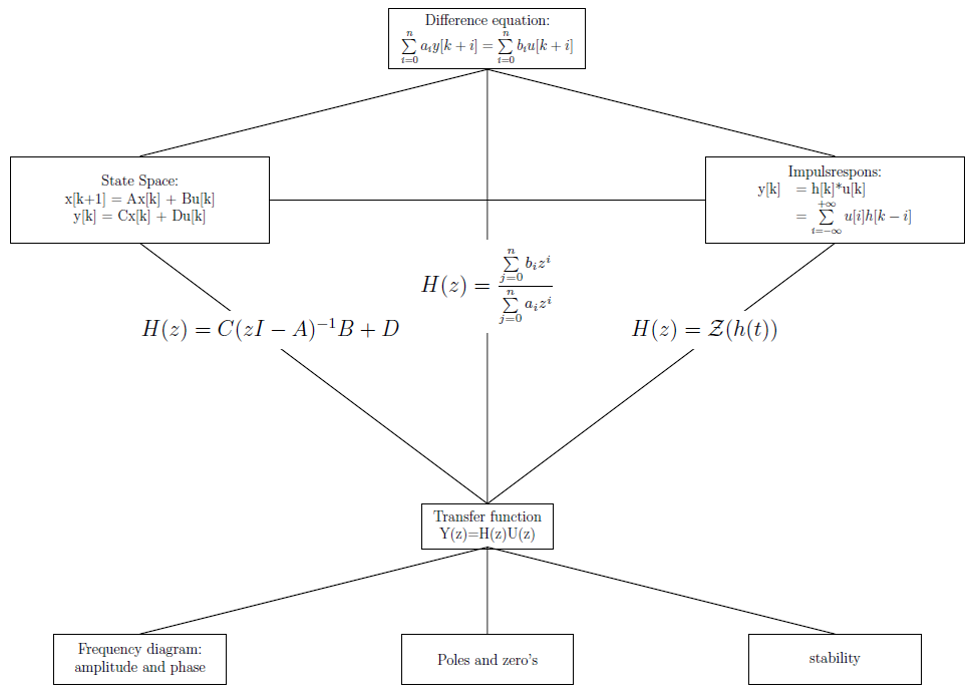
\includegraphics[width=0.7\linewidth]{Images/discrete_time_systems_28}
		\label{fig:discrete_time_systems_28}
	\end{figure}
\end{frame}
